\section{ТЕОРЕТИЧЕСКИЕ СВЕДЕНИЯ}

\subsection{Назначение и программная модель сопроцессора}

Математический сопроцессор --- устройство для обработки чисел с плавающей точкой.
Сопроцессор реализует поддержку различных представлений вещественных чисел,
арифметики с плавающей точкой, алгоритмов вычислений значений математических функций.

Программная модель сопроцессора представлена на рисунке~\ref{pic:program_model}.

\begin{figure}[h!]
  \centering
  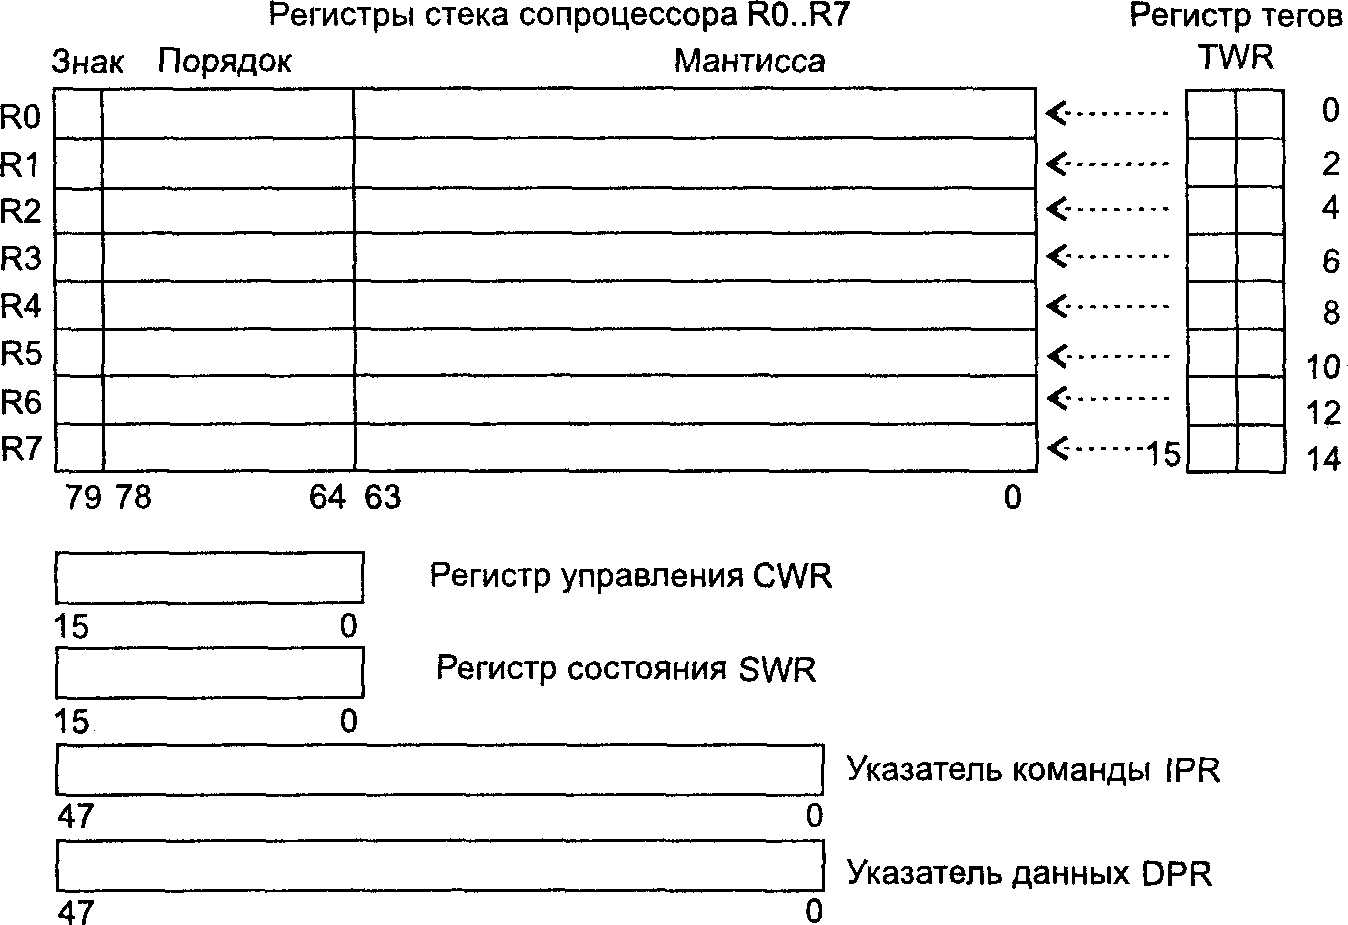
\includegraphics[width=0.8\linewidth]{pic/program_model}
  \caption{Программная модель сопроцессора}
  \label{pic:program_model}
\end{figure}

В этой модели можно выделить три группы регистров:
\begin{itemize}
\item регистры R0\dots R7 --- стек сопроцессора;
\item SWR, CWR, TWR --- служебные регистры;
\item DPR, IPR --- регистры указателей.
\end{itemize}

Регистры R0\dots R7 имеют размер по 80 битов и используются для
хранения и обработки вещественных данных.

Регистр SWR отражает информацию о текуцем состоянии сопроцессора и
содержит поля, позволяющие определить, какой регистр является текущей вершиной
стека, а также какие исключения возникли после выполнения последней команды.

Регистр CWR управляет режимами работы сопроцессора, с помощью полей в этом регистре
можно управлять точностью выполнения вычислений, управлять округлением маскировать исключения.

Регистр TWR используется для контроля состояния каждого из регистров R0\dots R7.

Регистры указателей предназначены для запоминания информации об адресе команды, вызвавшей 
исключительную ситуацию, и адресе её операнда.

\subsection{Описание команд сопроцессора}

Большое число команд сопроцессора обусловлено разнообразием входных данных.
Сопроцессор способен обрабатывать целые и вещественные числа в двоичном виде,
а также упакованные BCD (десятичные) числа.

Рассмотрим наиболее часто используемые семейства команд сопроцессора.

FINIT --- команда инициализации сопроцессора.

F(I,B)LD source --- загрузка вещественного (целого, десятичного) 
числа из памяти на вершину стека сопроцессора.

F(I,B)ST(p) destintation --- выгрузка вещественного (целого, десятичного) 
числа в память с вершины стека сопроцессора. Команды с префиксом <<p>>
отличаются тем, что дополнительно осуществляют очистку вершины стека.

F(I)ADD source --- команда сложения содержимого вершины стека с вещественным (целым)
аргументом. Результат операции помещается на вершину стека.

F(I)SUB source --- команда вычитания вещественного (целого)
аргументом из содержимого вершины стека. Результат операции помещается на вершину стека.

F(I)MUL source --- команда умножения содержимого вершины стека на вещественным (целым)
аргумент. Результат операции помещается на вершину стека.

F(I)DIV source --- команда деления содержимого вершины стека на вещественный (целый)
аргумент. Результат операции помещается на вершину стека.